\documentclass[10pt,a4paper]{article}
\usepackage[a4paper,vmargin={30mm,30mm},hmargin={30mm,30mm}]{geometry}
\usepackage[utf8]{inputenc}
\usepackage[slovak]{babel}
\usepackage{graphicx}
\usepackage{amsmath}
\usepackage{amssymb}
\usepackage{caption}
\usepackage{amsfonts}
\usepackage{booktabs}	
\usepackage{multicol}
\author{Jozef Urbanovský}
\title{Semestrálny projekt - Elektronika pre informačné technológie}

\begin{document}
\begin{titlepage}
	\begin{center}
	
        
\includegraphics[clip, width=4.0cm]{FIT.png}\\
    	\vspace*{3.0cm}
    	\huge{\textbf{Elektronika pre informačné technológie}}\\
    	\vspace*{1.0cm}
    	\huge{Semestrálny projekt}
    	\vspace*{0.5cm}\\
    	2015/2016\\
    	\vspace*{8.0cm}
	\end{center}


	\begin{minipage}{0.32\textwidth}
		\begin{center}
    		\textbf{\large Jozef Urbanovský\\(xurban66)}\\
		\end{center}
	\end{minipage}
	\hfill
	\begin{minipage}{0.32\textwidth}
		\begin{center}
    		\textbf{\large 21. Decembra 2015}\\
		\end{center}
	\end{minipage}	

\end{titlepage}	


\begin{titlepage}
    \tableofcontents
\end{titlepage}




 \section {Príklad 1}
 
 \subsection*{Zadanie}
 Stanovte napětí $U_{R3}$ a proud $I_{R3}$. Použijte metodu postupného zjednodušování obvodu.
\begin{center}
    \begin{tabular}{ | l | l | l | l | l | l | l | l | l | l | }
    \hline
    sk. & U[V] & R1[$\Omega$] & R2[$\Omega$] & R3[$\Omega$] & R4[$\Omega$] & R5[$\Omega$] & R6[$\Omega$] & R7[$\Omega$] & R8[$\Omega$]\\ \hline
    G & 130 & 380 & 420 & 330 & 440 & 450 & 650 & 410 & 275\\ \hline
    \end{tabular}
\end{center}

\vspace*{1cm}

\subsection*{Schéma obvodu}
 \begin{center}
    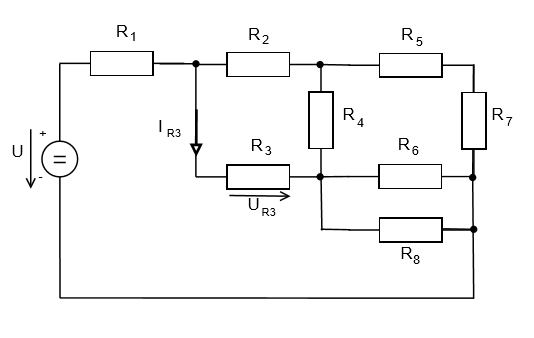
\includegraphics[clip, width=10cm]{1.png}
 \end{center}

 
\subsection*{Riešenie}
    \begin{enumerate}
        \item Pomocou metódy postupného zjednodušovania vyjadríme hodnotu celkového odporu rezistorov $R_{ekv}$ obvodu.
        \item Pomocou Ohmovho zákona vypočítame prúd $I$, ktorý prechádza obvodom.
        \item Opačným postupom vypočítame napätie $U_{R3}$ a prúd $I_{R3}$.
    \end{enumerate} \vspace*{1.5cm}

    
$R_{A}=\dfrac{R_{2}.R_{3}}{R_{2}+R_{3}+R_{4}} = 116.4706\Omega$ \vspace*{0.5cm}

$R_{B}=\dfrac{R_{2}.R_{4}}{R_{2}+R_{3}+R_{4}} = 155.2941\Omega$ \vspace*{0.5cm}

$R_{C}=\dfrac{R_{3}.R_{4}}{R_{2}+R_{3}+R_{4}} = 122.0168\Omega$ \vspace*{0.5cm}

\newpage
$R_{1A}=R_{1}+R_{A}=R_{1} + \dfrac{R_{2}.R_{3}}{R_{2}+R_{3}+R_{4}} = 496.4706\Omega$\\

\vspace*{0.5cm}

$R_{57}=R_{5}+R_{7}=860\Omega$ 

\vspace*{0.5cm}
	
$R_{68}=\dfrac{R_{6}.R_{8}}{R_{6}+R_{8}}=193.2432\Omega$

\vspace*{0.5cm}

$R_{B57}=R_{B}+R_{57}=R_{5}+R_{7}+\dfrac{R_{2}.R_{4}}{R_{2}+R_{3}+R_{4}} = 1015.2961\Omega$

\hspace*{0.5cm}

\vspace*{0.5cm}

$R_{C68}=R_{C}+R_{68}=\dfrac{R_{6}.R_{8}}{R_{6}+R_{8}} + \dfrac{R_{3}.R_{4}}{R_{2}+R_{3}+R_{4}} = 315.26\Omega$    

\hspace*{0.5cm}

\vspace*{0.5cm}

$R_{X}=\dfrac{R_{C68}.R_{B57}}{R_{C68}+R_{B57}}=
\dfrac
{
(\dfrac{R_{6}.R_{8}}{R_{6}+R_{8}} + \dfrac{R_{3}.R_{4}}{R_{2}+R_{3}+R_{4}})
.(R_{5}+R_{7} + \dfrac{R_{2}.R_{4}}{R_{2}+R_{3}+R_{4}})
}
{
(\dfrac{R_{6}.R_{8}}{R_{6}+R_{8}} + \dfrac{R_{3}.R_{4}}{R_{2}+R_{3}+R_{4}})
+(R_{5}+R_{7} + \dfrac{R_{2}.R_{4}}{R_{2}+R_{3}+R_{4}})
} = 240.5628\Omega$

\hspace*{0.5cm}

\vspace*{0.5cm}

$ {R_{EKV}} = R_{1A}+R_{X}=737.0334\Omega$

\vspace*{0.5cm}

$I=\dfrac{U}{R_{EKV}}=\dfrac{125}{931,9453}=0,1764A$

\vspace*{0.5cm}

$-U+U_{R1}+U_{R2}+U_{R8}=0 \implies U_{R3}=U-U_{R1}-U_{R8}=\underline{36.953V}$

\vspace*{0.5cm}

$I_{R3}=\dfrac{U_{R3}}{R_{3}}=\underline{0.1119A}$






 

 \newpage
 \section {Príklad 2}
 
 \subsection*{Zadanie}
 Stanovte napětí $U_{R3}$ a proud $I_{R3}$.Použijte metodu Theveninovy věty.
\begin{center}
    \begin{tabular}{ | l | l | l | l | l | l | l | }
        \hline
        sk. & U[V] & R1[$\Omega$] & R2[$\Omega$] & R3[$\Omega$] & R4[$\Omega$] & R5[$\Omega$]\\ \hline
        A & 50 & 525 & 620 & 210 & 530 & 130 \\ \hline
    \end{tabular}
\end{center}

\subsection*{Schéma obvodu}
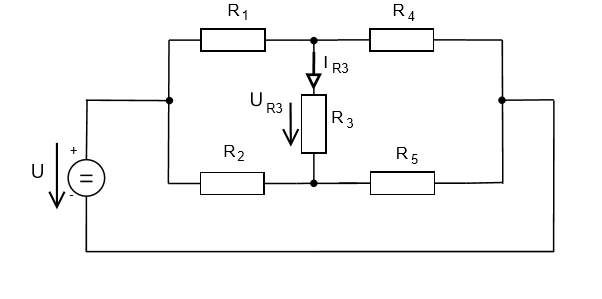
\includegraphics[clip, width=10cm]{2.png}


 \vspace*{0.5cm}
 
 \subsection*{Riešenie}
 \begin{enumerate}
\item Pomocou II.Kirchoffoveho zákona si zostavíme smyčky na vyjadrenie $U_{i}$
\item Spočítame hodnotu odporu $R_{i}$ - odporu medzi bodmi A,B (bez odporu $R_{3}$), pritom napätia sú ,,skratované".
\item Vypočítame veľkosť napätí $U_{R1}$ a $U_{R2}$, ktoré sa nachádzajú na rezistoroch v prvej smyčke.
\item Vypočítame hodnotu napätia $U_{i}$ naprázdno medzi bodmi A,B
\item Vypočítame prúd $I_{3}$ a napätie $U_{3}$
\end{enumerate}

\vspace*{0.5cm}
$U_{R1} + U_{i} - U_{R2} = 0 \implies U_{i} = U_{R2} - U_{R1}$
	
\vspace*{0.5cm}
	
$U_{i} + U_{R4} - U_{R5} = 0$

\vspace*{0.5cm}
    
$ R_{i}=\dfrac{R_{1}.R_{4}}{ R_{1}+R_{4}}+\dfrac{R_{2}.R_{5}}{R_{2}+R_{5}}=371.2108\Omega$
\vspace*{0.5cm}
    
$ U_{R1}=R1.\dfrac{U}{R_{1}+R_{4}}=24.8815 V$
    
\vspace*{0.5cm}
    
$U_{R2}=R2.\dfrac{U}{R_{2}+R_{5}}=41.53 V$
    
\vspace*{0.5cm}
    
$ U_{i}= U_{R2} - U_{R1} = 16.4518 V$

\vspace*{0.5cm}
    
\begin{center}
$ I_{R3} = \dfrac{U_{i}}{R_{i}+R_{3}}=\underline{0.0283 A}$ \qquad  \qquad $U_{R3}=R_{3}.I_{3}=\underline{5.9443 V}$
\end{center}

\vspace*{0.5cm}

 \newpage
 \section {Príklad 3}
 
 \subsection*{Zadanie}
 Stanovte napětí $U_{R3}$ a proud $I_{R3}$. Použijte metodu uzlových napětí ($U_{A}$, $U_{B}$,
$U_{C}$).
\begin{center}
    \begin{tabular}{ | l | l | l | l | l | l | l | l | l | }
    \hline
    sk. & U[V] & $I_{1}$[A] & $I_{2}$[A] & R1[$\Omega$] & R2[$\Omega$] & R3[$\Omega$] & R4[$\Omega$] & R5[$\Omega$] \\ \hline
    A & 120 & 0.9 & 0.7 & 530 & 490 & 650 & 390 & 320 \\ \hline
    \end{tabular}
\end{center}



\vspace*{1.5cm}   \subsection*{Schéma obvodu}
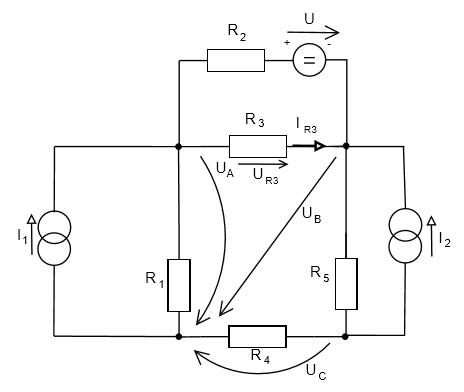
\includegraphics[clip, width=12cm]{3.png}


 \vspace*{0.5cm}
 
 \subsection*{Riešenie}
 \begin{enumerate}
\item Zostavíme rovnice pre uzly A,B,C podľa I. Kirchhoffovho zákona.
\item Zostavíme rovnicu pre každú vetvu s odporom a rovnice dosadíme do uzlových rovníc zostavených v predošlom bode.
\item Vypočítame veľkosť napätia $U_{A}$,$U_{B}$,$U_{C}$ naprázdno medzi bodmi A,B
\item Vypočítame prúd $I_{R2}$ a napätie $U_{R2}$
\end{enumerate}

\newpage

$A: I_{1}+I_{R2}-I_{R1}-I_{R3}=0  $

$B: I_{R3}+I_{2}-I_{R2}-I_{R5}=0  $

$C: I_{2}+I_{R4}-I_{R5}=0  $

\vspace*{0.5cm}
$ I_{R1}.R_{1}-U_{A}=0$\hspace*{2.7cm}
$\implies I_{R1}=\dfrac{U_{A}}{R_{1}}$
\vspace*{0.1cm}

$ I_{R2}.R_{2}-U+U_{A}-U_{B}=0$
\hspace*{1cm} 
$\implies I_{R2}=\dfrac{U+U_{B}-U_{A}}{R_{2}}$
\vspace*{0.1cm}

$ I_{R3}.R_{3}-U_{B}-U_{A}=0$\hspace*{1.8cm}
$\implies I_{R3}=\dfrac{U_{A}-U_{B}}{R_{3}}$
\vspace*{0.1cm}

$ I_{R4}.R_{4}-U_{C}=0$\hspace*{2.7cm}
$\implies I_{R4}=\dfrac{U_{C}}{R_{4}}$
\vspace*{0.1cm}

$ I_{R5}.R_{5}+U_{C}-U_{B}=0$\hspace*{1.8cm}
$\implies I_{R5}=\dfrac{U_{B}-U_{C}}{R_{5}}$
\vspace*{0.5cm}

$A: I_{1} + \dfrac{U+U_{B}-U_{A}}{R_{2}}-\dfrac{U_{A}}{R_{1}}-\dfrac{U_{A}-U_{B}}{R_{3}}=0$

\vspace*{0.3cm}
$B: \dfrac{U_{A}-U_{B}}{R_{3}}+I_{2}-\dfrac{U+U_{B}-U_{A}}{R_{2}}-\dfrac{U_{B}-U_{C}}{R_{5}}=0$

\vspace*{0.3cm}

$C: I_{2}+\dfrac{U_{C}}{R_{4}}-\dfrac{U_{B}-U_{C}}{R_{5}}=0  $

\vspace*{0.5cm}
Dostali sme 3 rovnice s 3 neznámymi, bude vhodné použiť maticu.
Do matice dosadíme známe \hspace*{0.5cm}hodnoty a upravujeme. \\

\[
\begin{pmatrix}
-9227 & 6042 & 0 \\ 3648 &-6833 & 3185 \\ 0 & -39 & 71 \\
\end{pmatrix}
\begin{pmatrix}
U_{A} \\ U_{B} \\ U_{C} \\
\end{pmatrix}
=
\begin{pmatrix}
-1932645 \\ -463840 \\ -8736 \\
\end{pmatrix}
\]

Po prevedení Gauss-Jordanovej eliminácie dostaneme jednoznačné výsledky v tvare :
\[
\begin{pmatrix}
1 & 0 & 0 \\ 0 &1 & 0 \\ 0 & 0 & 1 \\
\end{pmatrix}
\begin{pmatrix}
U_{A} \\ U_{B} \\ U_{C} \\
\end{pmatrix}
=
\begin{pmatrix}
\vspace*{0.1cm} \frac{7146891}{17321} \\ \vspace*{0.1cm}  \frac{5373886}{17321} \\ \frac{820638}{17321} \\
\end{pmatrix}
\]

\vspace*{0.5cm}
$ U_{A}=412.6142 V $

$ U_{B}= 310.2515 V $

$ U_{C}= 47.3782 V $

\vspace*{0.5cm}

\begin{center}
	$U_{R3} = U_{A} - U_{B} = \underline{102.3672 V} $ \qquad  \qquad
	$I_{R3} = \dfrac{U_{3}}{R_{3}} = \underline{0.1575 A} $
\end{center}


 \newpage
 \section {Príklad 4}
 
 \subsection*{Zadanie}
 Pro napájecí napětí platí: $u_{1}=U_{1}.sin(2\pi ft)$, $u_{2}=U_{2}.sin(2\pi ft)$.\\
 Ve vztahu pro napětí $ u_{C2}=U_{C2}.sin(2\pi ft + \varphi C_{2}) $ určete $|U_{C2}|$ a $\varphi _{C2}$. Použijte metodu smyčkových proudů.\\
 Pozn.: Pomocné "směry šipek napájecích zdrojů platí pro speciálny časový okamžik
 $\left( t=\dfrac{\pi}{2\omega}\right)$."\\
\begin{center}
    \begin{tabular}{ | l | l | l | l | l | l | l | l | l | l | }
    \hline
    sk.& $U_{1}$[V] & $U_{2}$[V] & $R_{1}$[$\Omega$] & $R_{2}$[$\Omega$] & $L_{1}$[mH] & $L_{2}$[mH] & $C_{1}$[$\mu$ F] & $C_{2}$[$\mu$ F]& $f$[Hz] \\ \hline
    F & 20& 35 & 120 & 100 & 170 & 80 & 150 & 90 & 65 \\ \hline
    \end{tabular}
\end{center}



\subsection*{Schéma obvodu}
    \begin{center}
        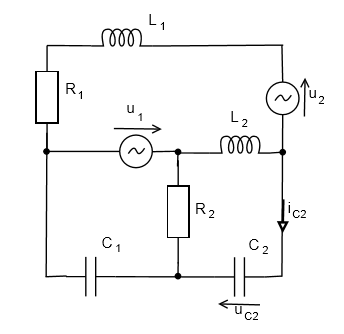
\includegraphics[clip, width=8cm]{4.png}
    \end{center}

 \vspace*{0.5cm}
 
 \subsection*{Riešenie}
 \begin{enumerate}
\item Vypočítame si impedanciu $Z_{1}$ až $Z_{5}$
\item Vytvoríme si slučky podľa II.Kirchoffoveho zákona na stanovenie rovníc pre každý prúd pretekajúci obvodom
\item Zostavíme si matice na výpočet prúdu $I_{C}$
\item Určíme amplitúdu napätia $U_{C2}$ a uhol $\varphi$
\end{enumerate}


\newpage
$Z_{1} = R_{1}+jX_{L1} \implies Z_{1} = R_{1}+j.2\pi fL_{1} = 120+69.4292j $ 

\vspace*{0.1cm}

$Z_{2} = jX_{L2} \implies Z_{2} = j.2\pi fL_{2} = 32.6726j $ 

\vspace*{0.1cm}

$Z_{3} = R_{2} = 100 $

\vspace*{0.1cm}

$Z_{4} = -jX_{C1} \implies Z_{4} = -j \frac{1}{j.2\pi fC_{1}} = -16.3236j $

\vspace*{0.1cm}

$Z_{5} = -jX_{C2} \implies Z_{5} = -j \frac{1}{j.2\pi fC_{2}} = -27.2060j $

\vspace*{0.5cm}

$I_{A}Z_{1}-U_{2}+(I_{A}-I_{C})Z_{2}-U_{1}=0$

\vspace*{0.1cm}

$I_{A}Z_{1}-U_{2}+I_{A}Z_{2} - I_{C}Z_{2} - U_{1}=0$

\vspace*{0.1cm}

$I_{A}(Z_{1}+Z_{2}) - I_{C}Z_{2} = U_{1}+U_{2}$

\vspace*{0.1cm}

$I_{A}(120+102.1018j) - I_{C}(32.6726j) = 55$

\vspace*{0.5cm}



$I_{B}Z_{4}+U_{1}+(I_{B}-I_{C})Z_{3}=0$

\vspace*{0.1cm}

$I_{B}Z_{4}+U_{1}+I_{B}Z_{3} - I_{C}Z_{3} =0$

\vspace*{0.1cm}

$I_{B}(Z_{3}+Z_{4}) - I_{C}Z_{3} = -U_{1}$

\vspace*{0.1cm}

$I_{B}(100-16.3236j) - I_{C}(100) =-20$

\vspace*{0.5cm}


$I_{C}Z_{5}+(I_{C}-I_{B})Z_{3}+(I_{C}-I_{A})Z_{2}=0$

\vspace*{0.1cm}

$I_{C}Z_{5}+I_{C}Z_{3}-I_{B}Z_{3}+I_{C}Z_{2}-I_{A}Z_{2}=0$

\vspace*{0.1cm}

$I_{C}(Z_{5}+Z_{3}+Z_{2})-I_{B}(Z_{3})-I_{A}(Z_{2})=0$

\vspace*{0.1cm}

$-I_{A}(32.6726j)-I_{B}(100)-I_{A}(100+5.4666j)=0$

\vspace*{0.5cm}


\[
M_{1}=
\begin{pmatrix}
120+102.1018j & 0 & -32.6726j \\ -32.6726j & -100 & 100+5.4666j \\ 0 & 100-16.3236j & -100 \\
\end{pmatrix}
\]\\

$|M_{1}| = ((120+102.1018j)(-100)(-100))+0+(-32.6726j)(-32.6726j)(100-16.3236j)-(0+0+(120+102.1018j)(100-16.3236j)(100+5.4666j)) = -228309.9543+138598.4108j$

\vspace*{0.5cm}

\[
M_{4}=
\begin{pmatrix}
120+102.1018j & 0 & 55 \\ -32.6726j & -100 & 0 \\ 0 & 100-16.3236j & -20 \\
\end{pmatrix}
\]\\

$|M_{4}| = ((120+102.1018j)(-100)(-20)+0+(55)(-32.6726j)(100-16.3236j))-(0+0+0) = 210666.6051+24504.2999j $

\newpage

$I_{C}=\frac{det(M_{4})}{det(M_{1})}$

\vspace*{0.1cm}

$I_{C}=\frac{210666.6051+24504.2999j}{-228309.9543+138598.4108j}$

\vspace*{0.1cm}

$I_{C} = I_{C2} =  -0.6266-0.4877j$

\vspace{0.5cm}

$U_{C2}= I_{C2}.Z_{5} $

\vspace*{0.1cm}

$U_{C2}= (-0.6266-0.4877).(-27.2060j) $

\vspace*{0.1cm}

$U_{C2}= -1.1143-27.206 i $

\vspace{0.5cm}

$\varphi{C2} = \pi - arctg(\dfrac{27.206}{1.1143})$

\vspace*{0.1cm}

$\varphi{C2} =\pi - 1.52986 rad $

\vspace*{0.1cm}

$\varphi{C2} = 1.61173 rad$

\vspace*{0.5cm}

$U_{m_{C2}} = |U_{C2}|$

\vspace*{0.1cm}

$U_{m_{C2}} = \sqrt{27.206^{2}+1.1143^{2}}$

\vspace*{0.1cm}

$U_{m_{C2}} = \underline{27.2288 V}$

\vspace*{0.5cm}

$\underline{U_{m_{C2}}=27.2288.sin(\omega t+1.61173 rad)}$



 


\newpage
 \section {Príklad 5}
 
 \subsection*{Zadanie}
 
 Sestavte diferenciální rovnici popisujúcí chování obvodu na obrázku, dále ji upravte dosazením hodnot parametru. Vypočítejte analytické řešení $u_{C}$ = f(t). Proveďte kontrolu výpočtu dosazením do sestavené diferencíalní rovnice.
\begin{center}
    \begin{tabular}{ | l | l | l | l | l |}
    	\hline
    	sk.& $U$[V] &  $C$[F] & $R$[$\Omega$] & $u_{C}(0)$[A]\\ \hline
    	A  & 20 &  40 & 10 & 9\\ \hline
    \end{tabular}
\end{center}



\vspace*{1.5cm}   \subsection*{Schéma obvodu}
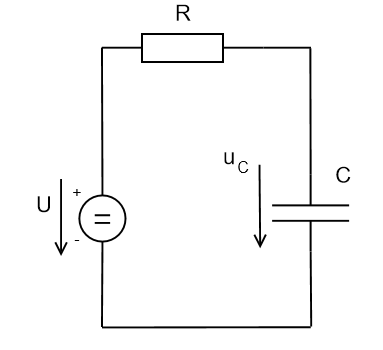
\includegraphics[clip, width=8cm]{5.png}


 \vspace*{0.5cm}
 
 \subsection*{Riešenie}
 \begin{enumerate}
\item Zostavíme rovnicu podľa II. Kirchhoffovho zákona pre obvod
\item Rovnicu dosadíme do axiómu a následne derivujeme
\end{enumerate}

\vspace*{0.5cm}

	$U_{R} + u_{C} - U = 0$
	
	\vspace*{0.1cm}
	
	$i = \dfrac{U - u_{C}}{R}$
	
	\vspace*{0.1cm}
	
	Axióm : $u_{C}' =\dfrac{1}{C}$
	
	\vspace*{0.1cm}
	
	$u_{C}' =\dfrac{U - u_{C}}{RC}$
	
	\vspace*{0.1cm}
	
	$u_{C}' =\dfrac{20 - u_{C}}{400}$
	
	\vspace*{0.1cm}
	
	$u_{C}' + \dfrac{1}{400}u_{C} = \dfrac{1}{40}$
	

	\newpage
	Zostavíme charakteristickú rovnicu
	\vspace*{0.1cm}
	
	$\lambda + \dfrac{1}{400} = 0$
	
	\vspace*{0.1cm}
	
	$\lambda = -\dfrac{1}{400}$
	
	\vspace*{0.1cm}

	Očakávaný tvar riešenia
	
	\vspace*{0.1cm}
	
	$u_{C}(t) = c(t)e^{\lambda t}$
	
	\vspace*{0.1cm}
	
	$u_{C}(t) = c(t)e^{-\frac{1}{400}t}$
	
	\vspace*{0.1cm}
	
	$u_{c}'(t) = c'(t)e^{-\frac{1}{400}t} + c(t)e^{-\frac{1}{400}t}.(-\frac{1}{400})$
	
	\vspace*{0.1cm}

	$u_{c}'(t) + \frac{1}{400} u_{C}(t) = \frac{20}{400}$

	\vspace*{0.1cm}
	
	$c'(t)e^{-\frac{1}{400}t} - c(t)e^{-\frac{1}{400}t} + c(t)e^{-\frac{1}{400}t} = \frac{20}{400}$

	\vspace*{0.1cm}
	
	$c'(t)e^{-\frac{1}{400}t} = \frac{20}{400}$
	
	\vspace*{0.1cm}
	
	$c'(t) = \frac{20}{400}e^{\frac{1}{400}t}$
	
	\vspace*{0.1cm}
	
	$\int c'(t)dt = \int \frac{20}{400}e^{\frac{1}{400}t}dt$

	\vspace*{0.1cm}
	
	$c(t)+K_{1} = \frac{20}{400}.400.e^{\frac{1}{400}t}+K_{2}$
	
	\vspace*{0.1cm}
	
	$c(t) = 20.e^{\frac{1}{400}t}+K$
	
	\vspace*{0.1cm}
	
	$u_{C}(t) = (20.e^{\frac{1}{400}t}+K).e^{-\frac{1}{400}t}$
	
	\vspace*{0.1cm}
	
	$u_{C}(t) = 20+K.e^{-\frac{1}{400}t}$
	
	\vspace*{0.3cm}
	
	Pre $u_{C}(0) = 9$
	
	\vspace*{0.1cm}
	
	$u_{C}(0) = 20 + K$
	
	\vspace*{0.1cm}
	
	$9 = 20 + K$
	
	\vspace*{0.1cm}
	
	$-11 = K$
	
	\vspace*{0.1cm}
	
	$u_{C}(t) = 20 - 11.e^{-\frac{1}{400}t}$
	
	
	

\newpage
 \section {Tabuľka výsledkov}
 \begin{center}
 \renewcommand{\arraystretch}{2}
    \begin{tabular}{ | l | l | l |  }
    \hline
    Číslo príkladu & Skupina &  Výsledky \\ \hline
    1 & G & $U_{R3}=36.953V$ 
    $I_{R3}=0.1119A$ \\ \hline
    2 & A & $ I_{R3} = 0.0283 A$ $U_{R3}=5.9443 V$ \\ \hline
    3 & A & $ U_{A}=412.6142 V $
    $ U_{B}= 310.2515 V $    
    $ U_{C}= 47.3782 V $ \\ \hline
    4 & G & $U_{m_{C2}}=27.2288.sin(\omega t+1.61173 rad)$ \\ \hline
    5 & A & $u_{C}(t) = 20 - 11.e^{-\frac{1}{400}t}$ \\ \hline
    \end{tabular}
\end{center} 
 
\end{document}\documentclass[11pt]{article}
